\subsection{Dreiecksgenerator}
\begin{figure}[H]
\centering
 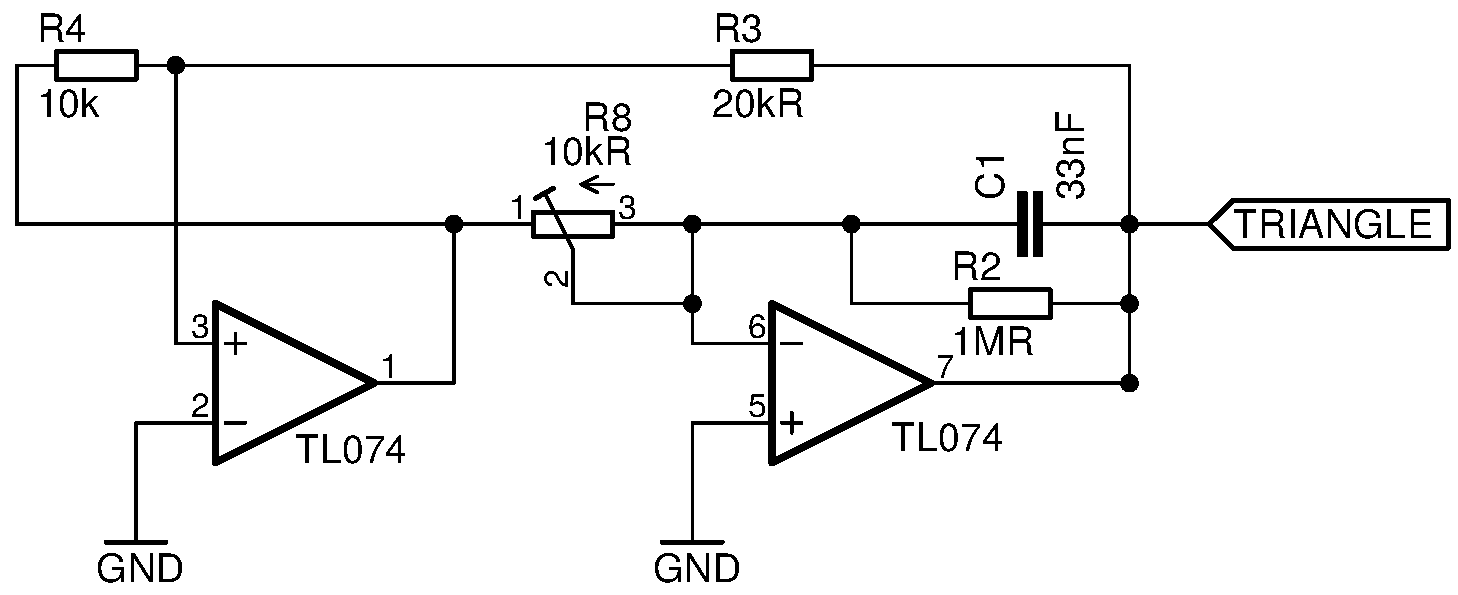
\includegraphics[scale=1]{gfx/triangle_generator.pdf}
 \caption{Miller Integrator}
	\label{triangle} 
\end{figure}
Für die Generierung eines Dreiecksignals wurde ein Miller-Integrator verwendet.
Die Grundlage für die Schaltung liegt in einer Applicationnote von TI\footnote{ Texas Instruments,Appnote 20, Seite 24, www.ti.com/lit/an/snoa621c/snoa621c.pdf}
Das Grundprinzip dieser Schaltung besteht aus einem Intergrator, welcher auf einen invertierenden Schmitt-Trigger rückgekoppelt ist.
Der linke Operationsverstärker bildet mit $R_4$ und $R_3$ den Schmitt-Trigger. Der Integrator besteht aus $R_8$,$C_1$ und dem rechten Operationsverstärker in Abbildung \ref{triangle}.
Frequenzbestimmend sind in dieser Schaltung alle Bauteile. Durch $R_4$ und $R_3$ werden die Schaltschwellen, und damit die Amplitude bestimmt. Diese berechnet sich wie folgt: 
\begin{equation}
U_H = \pm\frac{R_3}{R_4}\cdot V_{cc}
\end{equation}
Mit $R_8$ und $C_1$ wird die Flankensteilheit($k$) in $\frac{V}{s}$ bestimmt:
\begin{equation}
k=\frac{V_{cc}}{R_8 \cdot C_1}
\end{equation}
Die Frequenz des Dreieckssignals berechnet sich zu:
\begin{equation}
f = \frac{R_4}{4 \cdot R_8 \cdot R_3 \cdot C_1}
\end{equation}
$C_1$ wurde mit $33nF$ fest gewählt. $U_{ein}$ ist die Betriebspannung($V_{cc}$), welche mit $9V$ gewählt wurde.